\documentclass[a4paper,12pt]{article}
\usepackage[a4paper,top=1.3cm,bottom=2cm,left=1.5cm,right=1.5cm,marginparwidth=0.75cm]{geometry}
\usepackage{setspace}
\usepackage{cmap}
\usepackage{mathtext}
\usepackage[T2A]{fontenc}
\usepackage[utf8]{inputenc}
\usepackage[english,russian]{babel}
\usepackage{multirow}
\usepackage{graphicx}
\usepackage{wrapfig}
\usepackage{tabularx}
\usepackage{float}
\usepackage{longtable}
\usepackage{hyperref}
\hypersetup{colorlinks=true,urlcolor=blue}
\usepackage[rgb]{xcolor}
\usepackage{amsmath,amsfonts,amssymb,amsthm,mathtools}
\usepackage{icomma}
\mathtoolsset{showonlyrefs=true}
\usepackage{euscript}
\usepackage{mathrsfs}
\usepackage{float}
\setlength{\parindent}{1cm} % Устанавливает отступ в 1.5 см для всех абзацев


\DeclareMathOperator{\sgn}{\mathop{sgn}}
\newcommand*{\hm}[1]{#1\nobreak\discretionary{}
	{\hbox{$\mathsurround=0pt #1$}}{}}

\title{\textbf{Отчёт о выполненой лабораторной работе \\ \textit{Определение $C_p / C_v$ методом адиабатического расширения (2.1.2)}}}

\author{Каплин Артём Б01-402}
\date{23 марта 2025}

\begin{document}
\maketitle

\subparagraph*{Цель работы:}определение отношения $C_p / C_v$ для воздуха и углекислог газа.
\subparagraph*{В работе используются:}стеклянный сосуд: U-образный жидкостный манометр; резиновая груша; газгольдер с углекислым газом, секундомер. 

\section{Экспериментальная установка}

Экспериментальная установка состоит из стеклянного сосуда $A$, снабжённого краном $K_1$, и U-образного жидкостного манометра, измеряющего избыточное давление газа в сосуде. Схема установки показана на рисунке:

\begin{center}
    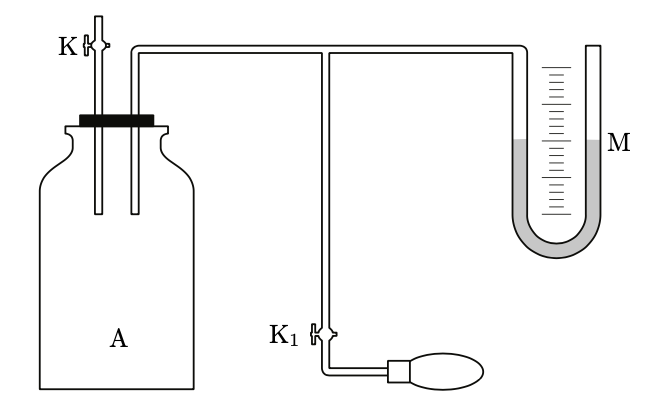
\includegraphics[width=0.5\textwidth]{ust.jpg}
\end{center}

С помощью резиновой груши, соединённой трубкой и краном $K_1$, в сосуде создаётся избыточное давление воздуха. При этом газ оказывается перегретым по отношению к окружающей среде. Будем следить за изменением его давления вследствие теплообмена со стенками сосуда: через некоторое время газ остынет до комнатной температуры (изохорное охлаждение). При этом давление воздуха понизится до $p_0 + \Delta p_1$, где

\begin{equation}
    \Delta p_1 = \rho g \Delta h_1.
\end{equation}

Откроем кран $K_2$, за время $\Delta t$ порядка 0.5 с происходит адиабатическое расширение газа, и его температура окажется ниже комнатной. Далее газ будет изобарически нагреваться . Зададим время $\tau$, в течение которого кран $K_2$ остаётся открытым, таким чтобы можно было пренебречь временем $\Delta t$ адиабатического расширения воздуха. После закрытия крана $K_2$ газ станет изохорически нагреваться до комнатной температуры, при чём давление внутри сосуда возрастёт до $p_0 + \rho g \Delta h_2,$ где

\begin{equation}
    \Delta p_2 = \rho g \Delta h_2.
\end{equation}

Наибольший интерес представляет исследование зависимости отношения перепадов давления $\frac{\Delta p_1}{\Delta p_2}$ от времени $\tau$. \\



С хорошей точностью мы можем считать воздух в газгольдере идеальным газом. Рассмотрим изобарическое расширение воздуха. Для этого запишем уравнение теплового баланса для имеющейся во времени массы газа: $m = \frac{p_0V_0}{RT}\mu$:

\begin{equation}
    c_p m \ dT = -\alpha (T - T_0) dt, 
\end{equation}

где $c_v$ — удельная теплоёмкость воздуха при постоянном давлении, $a$ — положительный постоянный коэффициент, характеризующий теплообмен, $V$ — объем сосуда.

Перепишем уравнение в виде:

\begin{equation}
    \frac{dT}{T(T - T_0)} = -\frac{\alpha dt}{c_p \frac{p_0V_0}{R}\mu} 
\end{equation}

После преобразования:

\begin{equation}
    \frac{1}{T_0} \left(\frac{1}{T} -\frac{1}{T - T_0} \right)dT = -\frac{\alpha dt}{c_p m_0T_0} 
\end{equation}

После сокращения на $T_0 $ выполним интегрирование:
\begin{equation}
    \int \frac{1}{T_0} \left(\frac{1}{T} -\frac{1}{T - T_0} \right)dT = -\frac{\alpha}{c_p m_0T_0} \int dt
\end{equation}

\begin{equation}
    \ln \left( \frac{T_2 \cdot \Delta T_1}{T_1 \cdot \Delta T_2} \right) =  \frac{a}{c_p} \tau
\end{equation}

Для адиабатического расширения справедливо соотношение $T^{\gamma} = const \cdot p^{\gamma-1}$. После взятия логарифмических производных, получим:

\begin{equation}
    \gamma \frac{dT}{T} = (\gamma - 1) \frac{dp}{p}
\end{equation}

Переходя к конечным приращениям:

\begin{equation}
    \frac{\Delta T}{T} = \frac{\gamma - 1}{\gamma} \frac{\Delta p_1}{p_0}
\end{equation}

При изохорическом нагреве выполняется: $\frac{p}{T} = \text{const}$. Возьмём от этого выражения логарифмическую производную: $\frac{dp}{p} = \frac{dT}{T}$. В конечных приращениях $\frac{\Delta T_2}{T_2} = \frac{\Delta p_2}{p_0}$.

После подстановок получаем:
\begin{equation}
    \left( \frac{\gamma - 1}{\gamma} \right) \frac{\Delta p_1}{p_0} = \frac{\Delta p_2}{p_0} \exp\left(\frac{\alpha}{c_p m_0}\right)
\end{equation}


Подставляя первые выражения, получаем:

\begin{equation}
    \frac{\Delta h_1}{\Delta h_2} = \frac{\gamma}{\gamma - 1} \exp \left( \frac{\alpha}{c_p m_0}  \tau\right) 
\end{equation}

Следовательно, 

\begin{equation}
    \ln{\frac{\Delta h_1}{\Delta h_2}} = \ln{\frac{\gamma}{\gamma - 1}} + \left( \frac{\alpha}{c_p m_0}  \tau\right) 
\end{equation}

Из графика зависимости $\ln{\frac{\Delta h_1}{\Delta h_2}}$ от $\tau$ определим $\gamma$.
 

\section{Ход работы}

\begin{enumerate}
    \item Проверим исправность установки. Перед началом работы убедимся в том, что краны и места сочленений трубок достаточно герметичны. Убедимся, что давление через некоторое время установится.
    \item Закроем краны $K_1$ и $K_2$, убедимся что уровни жидкости в манометре одинаковы.
    \item Откроем кран $K_1$ (в случае воздуха используем резиновую грушу), наполним сосуд газом так, чтобы разность уровней жидкости в манометре составляла примерно у воздуха 20-25 см, а у углекилого газа 8-12 см (так как больше газгольдер не выдаёт).
    \item Закроем кран  $K_2$. После того как давлене в сосуде перестанет изменяться, измерим разность уровней жидкости $\Delta h_1$ в манометре.
    \item Откроем кран $K_2$ на время $\tau$ в интервале 5-35 с.
    \item После того как давлене в сосуде перестанет изменяться, измерим разность уровней жидкости $\Delta h_2$ в манометре.
    \item Откроем краны $K_2$ и $K_1$ на 3–4 минуты.
    \item Повторим действия, перечисленные выше  несколько раз для разного времени $\tau$.

\end{enumerate}


\subsection{Измерения для воздуха}

Измерения проходили при таких параметрах в комнате: давление  $P = 101,325$ кПа, температура в комнате $T = 297$ K, влажность $\varphi = 91 \%$.

\[
z = \ln\left(\frac{\Delta h_1}{\Delta h_2}\right)
\]

\[
\sigma_z = \sigma_{\Delta h} \cdot \sqrt{\left( \frac{1}{\Delta h_1} \cdot  \right)^2 + \left( \frac{1}{\Delta h_1} \right)^2 }
\]


\begin{table}[h!]
    \caption{Экспериментальные данные для воздуха $\Delta t$}
    \begin{center}
    \begin{tabular}{|l|l|l|l|l|l|l|}
        \hline
        № & $\Delta h_1$ , см & $\Delta h_2$, см & $\tau$, с & $\ln{\frac{\Delta h_1}{\Delta h}}$ & $\sigma_z$ & $\frac{\sigma_z}{z} \cdot 100\%$ \\\hline
        1 & 19.8 & 4.2 & 5  & 1.551 & 0.049 & 3.16 \\\hline
        2 & 17.2 & 3.4 & 6  & 1.621 & 0.060 & 3.70 \\\hline
        3 & 18.3 & 3.2 & 8  & 1.744 & 0.063 & 3.61 \\\hline
        4 & 20.4 & 3.0 & 12 & 1.917 & 0.067 & 3.50 \\\hline
        5 & 21.7 & 2.4 & 18 & 2.202 & 0.084 & 3.81 \\\hline 
        6 & 20.9 & 1.8 & 24 & 2.452 & 0.112 & 4.57 \\\hline
        7 & 20.9 & 1.4 & 29 & 2.703 & 0.143 & 5.29 \\\hline
        8 & 21.6 & 1.1 & 34 & 2.977 & 0.182 & 6.11 \\\hline
    \end{tabular}
    \end{center}
\end{table}

\begin{figure}[h!] 
    \centering
    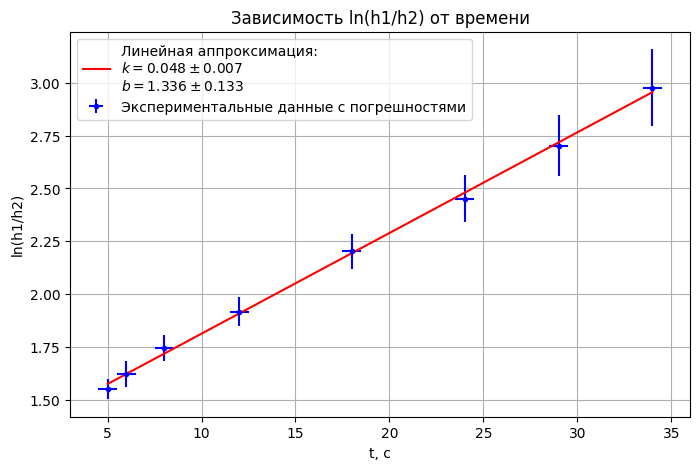
\includegraphics[width=0.9\linewidth]{1.png} 
    \caption{График зависимости $h(t)$}
    \label{plan2} 
\end{figure}

Lля нахождения \(\gamma\) по известному значению \(b\), можно подставить значение \(b\) в формулу:

\[
\gamma = \frac{e^b}{e^b - 1},
\]
где \(b\) выражается как:

\[
b = \ln{\frac{\gamma}{\gamma - 1}}
\]

Из графика коэфициент $b = 1.336 \pm 0.133$. Тогда $\gamma = 1.357 \pm 0.064$, $\varepsilon_{\gamma} = 4,74 \%$. 


\subsection{Измерения для для углекислого газа}

\begin{table}[h!]
    \caption{Экспериментальные данные для углекислого газа $\Delta t$}
    \begin{center}
    \begin{tabular}{|l|l|l|l|l|l|l|}
        \hline
        № & $\Delta h_1$ , см & $\Delta h_2$, см & $\tau$, с & $\ln{\frac{\Delta h_1}{\Delta h}}$ & $\sigma_z$ & $\frac{\sigma_z}{z} \cdot 100\%$ \\\hline
        1 & 9.2 & 2.4 & 5  & 1.344 & 0.086 & 6.41 \\\hline
        2 & 8.8 & 1.2 & 10 & 1.992 & 0.168 & 8.43 \\\hline
        3 & 9.4 & 1.0 & 15 & 2.241 & 0.201 & 8.97 \\\hline
        4 & 9.0 & 0.9 & 20 & 2.303 & 0.223 & 9.68 \\\hline
        5 & 8.9 & 0.7 & 25 & 2.543 & 0.287 & 11.29 \\\hline 
        6 & 8.7 & 0.4 & 30 & 3.080 & 0.501 & 16.26 \\\hline
        7 & 8.7 & 0.4 & 35 & 3.080 & 0.501 & 16.26 \\\hline
    \end{tabular}
    \end{center}
\end{table}

\begin{figure}[h!] % Изменяем на [h!] для контроля расположения
    \centering
    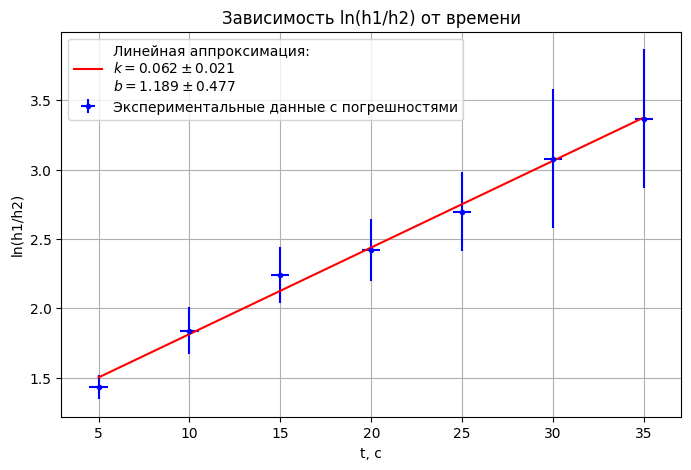
\includegraphics[width=0.9\linewidth]{3.png} % Уменьшена ширина
    \caption{График зависимости $h(t)$}
    \label{plan2} % Перенесено после \caption
\end{figure}

У углекислого газа коэфициент $b = 1.189  \pm 0.477$. Тогда $\gamma = 1.438 \pm 0.300$, $\varepsilon_{\gamma} = 20 \%$.

\newpage
	\section{Вывод}
	
	В ходе лабораторной работы было получено значение показателя адиабаты для воздуха и углекислого газа. Сравним реультаты эксперимента с табличными значениями, взятыми с книги Лабораторный практикум по общей физике. Табличные значения взяты при $T = 20 ^\circ C$ для сухого воздуха и углекислого газа.


\begin{table}[h!]
    \centering
    \begin{tabular}{|c|c|c|c|c|}
        \hline
            & $\gamma^{\text{эксп}}$ & $\gamma^{\text{табл}}$ & $\sigma_{\gamma}$ & $\varepsilon_{\gamma}, \%$ \\ \hline
        Воздух & $1.357$ & $1.40$ & $0.064$  &  $4.74$  \\ \hline
        CO$_2$ & $1.438$ & $1.30$ & $0.300$ & $20$  \\ \hline
    \end{tabular}
    \caption{Сравнение экспериментальных и табличных значений $\gamma$ для различных газов}
\end{table}
    
 Неполное совпадение результата вызвано, во-первых, погрешностью в определении времени $\tau$, а во-вторых с тем, что снятая мной разница уровней воды в трубке не всегда была точной, так как время на выполнение работы ограничено. Так мы видим, что погрешность у углекислого газа оказалась значительной, могу предположить, что это связанно как раз таки с тем, что последние точки снимались быстро, из-за чего газ мог не возвращаться в состояние равновесия.
	

\end{document}
